\section{问题提出的背景}

\subsection{背景介绍}
\par 随着经济和科技的发展,人们越来越关注自己的健康问题,而宫颈癌在女性常见的癌症中发病率高居第四位,可谓女性健康的重大威胁。2018年,全球估计有57万女性被诊断出患有宫颈癌,约31.1万女性死于该疾病。然而,宫颈癌并非不能通过预先的检查发现,全世界大约七成的宫颈癌发生在发展中国家\cite{wild2014world},在发达国家中,就是因为宫颈抹片筛查以及其他检测方法的普及,宫颈癌的发病率和致死率大大降低\cite{canavan2000cervical}。由此,定期进行科学的宫颈抹片等筛查诊断是十分必要的。
\par 宫颈癌筛查主要由“细胞学-阴道镜-组织学”三阶梯诊断程序组成,其中,细胞学筛查的主要手段就是TCT检查,即采用液基薄层细胞检测系统检测宫颈细胞并进行细胞学分类诊断。诊断通常需要医生通过多个复杂的步骤制作患者的宫颈细胞涂片,并在显微镜下通过估计细胞的类型和形态特征,如细胞核大小、核胞浆比等寻找疑似病变或病变细胞,最后根据全片病变细胞的状况给出诊断。
\par 对医生来说,分析TCT检查的片子非常耗时费力,并且诊断结果可能存在一定的主观性,由于医生的精力等原因可能造成漏诊或误诊,不利于医生准确把握患者的病情,并依此展开进一步的治疗。由此,亟需引入计算机的辅助诊断方法帮助医生实现快速、准确的宫颈癌筛查。
\subsection{本研究的意义和目的}
\par 本研究希望通过计算机辅助医生完成TCT检查的过程,如\ref{检测}所示,通过计算机自动识别并标注涂片上的病变细胞并将它们分为不同的病变等级,以此实现快速、准确的宫颈癌筛查。
\begin{figure}[h]
    \centering
    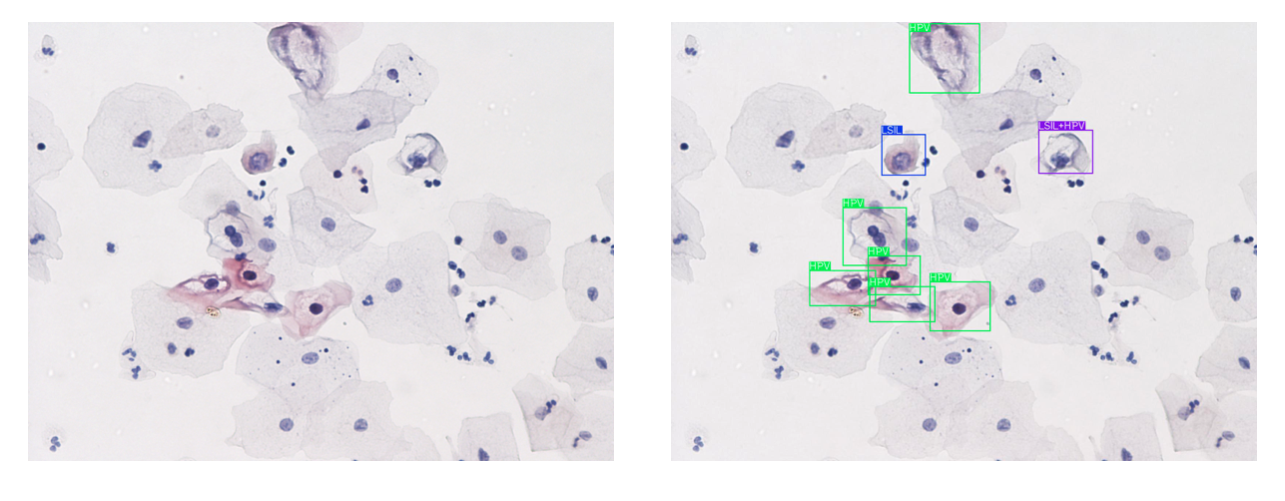
\includegraphics[width=0.5\paperwidth]{TCT/example_dete.png}
    \caption{计算机辅助检测样例,左图为输入图片,右图为计算机辅助检测的结果,标注出了所以的病变细胞并为每个病变细胞诊断病变等级}
    \label{检测}
\end{figure}

\par 在临床实践的过程中,TCT检查可能会遇到许多问题。首先,涂片在显微镜的视野下十分巨大,整个TCT样本的片子含有几亿甚至几十亿像素,涂片上也有上亿细胞,医生几乎不可能逐一筛查病变细胞;其次,在判定病变细胞等级的时候,医生的主观偏好可能会影响检查结果,这将十分不利于医生和患者获知准确的病情并依此展开治疗。由此,我们希望通过计算机的辅助极大地减少医生的工作量,避免诊断过程中因为人为原因造成遗漏等问题,并进一步提高诊断结果的准确性。
